
%(BEGIN_QUESTION)
% Copyright 2007, Tony R. Kuphaldt, released under the Creative Commons Attribution License (v 1.0)
% This means you may do almost anything with this work of mine, so long as you give me proper credit

Observing this process trend, we see the PV, SP, and Output variables represented:

$$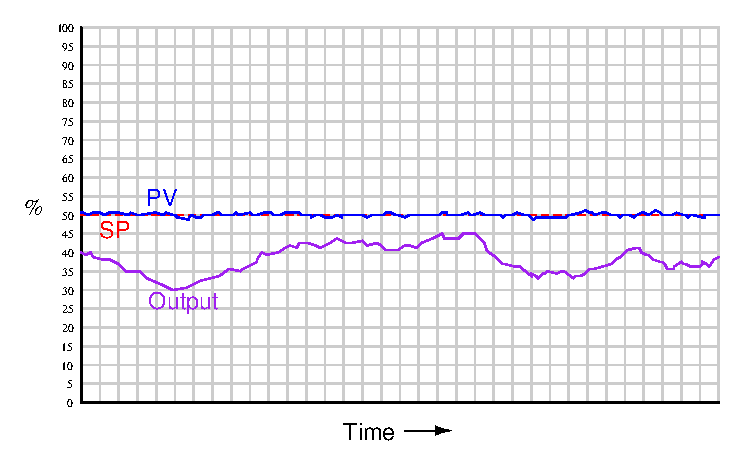
\includegraphics[width=15.5cm]{i01647x01.eps}$$

The setpoint (SP) is the flat line at 50\%.  The process variable (PV) is the slightly bumpy plot wavering just above and below the flat setpoint line.  The output is the very erratic plot below both PV and SP plots.

The operator of this process calls you, the technician, to complain about the quality of control in this process.  He claims the controller needs to be tuned in order to stabilize the Output plot so that it is not so erratic.  Based on your observations of this trend, what do you think is happening with this process?  Is the controller in need of tuning?
 
\vskip 10pt

What do you think might happen if we placed this controller in ``manual'' mode?  How would that change the appearance of the process trend?

\vfil 

\underbar{file i01647}
\eject
%(END_QUESTION)





%(BEGIN_ANSWER)

This is a graded question -- no answers or hints given!

%(END_ANSWER)





%(BEGIN_NOTES)

There is nothing wrong with the tuning of the controller in this process.  The combination of stable PV trend and erratic output trend indicates that the controller is doing exactly what it is supposed to: keeping the process variable at setpoint, by adjusting the manipulated variable accordingly.

What is happening in this process is that we have a fluctuating process {\it load} forcing the controller to react ``erratically'' to maintain the PV equal to SP.  This is not the fault of the controller, but rather the process itself.

\vskip 10pt

After placing the controller in ``manual'' mode, the trend might appear something like this:

$$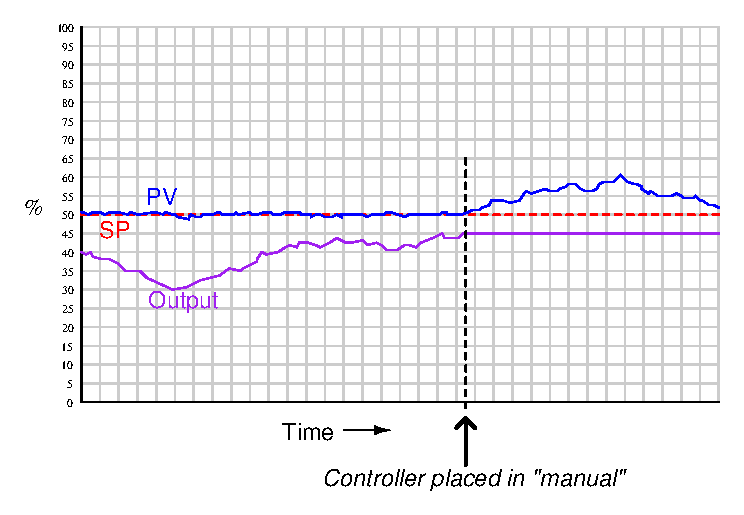
\includegraphics[width=15.5cm]{i01647x02.eps}$$

Having said this, it should be noted that the erratic output action of the controller will have detrimental effects on the control valve (if the final control element is a control valve), such as premature packing wear and leakage, and excessive compressed air consumption for pneumatic actuators (which is an ongoing expense!).  The only way to deter this, short of eliminating load variability in the process, is to de-tune the controller so it does not respond so aggressively to changes in PV.  However, the negative consequence of this is that the PV will not hold so close to setpoint any more.
 
Ultimately, the situation is this: so long as process load variability remains, you cannot have robust control (low PV $-$ SP error) {\it and} a steady output signal.  You can have one or the other (or neither!), but not both.

In manual mode, the Output plot turns into a flat line (because the controller simply holds the output value at whatever it was at the moment of auto-to-manual transition), and the PV is free to ``wander'' according to changes in process load.  Here, variations in process load reveal themselves clearly.

%INDEX% Control, PID tuning: manual mode as a diagnostic tool
%INDEX% Process troubleshooting: diagnosing problem via trend recording

%(END_NOTES)


